\documentclass[12pt, letterpaper]{article}
\usepackage[utf8]{inputenc}

\usepackage{geometry}
\geometry{
a4paper,
left=25mm,
right=25mm,
top=25mm,
bottom=25mm
}

% TODO: Do I want 1 or 2 columns?
\usepackage{multicol}

\usepackage{graphicx}
\graphicspath{ {images/} }
\usepackage{wrapfig}

\usepackage{textcomp}

\usepackage{hyperref}
\usepackage[all]{hypcap}

% Set the link style for the document.
\hypersetup{
colorlinks,
citecolor=blue,
filecolor=blue,
linkcolor=blue,
urlcolor=blue
}

\usepackage[explicit]{titlesec}

\titleformat{\paragraph}[runin]
{\normalfont\normalsize\bfseries}{\theparagraph}{1em}{#1\quad--}


% Start fix titlesec numbering.
\usepackage{etoolbox}
\makeatletter
\patchcmd{\ttlh@hang}{\parindent\z@}{\parindent\z@\leavevmode}{}{}
\patchcmd{\ttlh@hang}{\noindent}{}{}{}
\makeatother
% End fix titlesec numbering.


\providecommand{\keywords}[1]{\textbf{\textit{Keywords---}} #1}

% ==============================================================================



\title{Spectrangle}
\author{Wybe Westra --- s1578472}
\date{Software Systems \\ \today}

\begin{document}

    \maketitle

    \newpage

    \tableofcontents

    \newpage


    \section{Design}

    Spectrangle is implemented using a separate server and client.
    The game functionality is divided between the two according to the requirements laid out in the module manual,
    with one small exception.
    One cannot select a port for the server or client.
    This is because the network protocol determines that only port 4000 is to be used.

    Other than that, all the functionality required for single-person ``groups'' is implemented.

    % ------------------------------------------------------------------------------------------------------------------

    \subsection{Client and MVC}

    \begin{figure}[ht]
        \begin{center}
            \includegraphics[width=\textwidth]{Client.png}
            \caption{Diagram depicting how the client functions.
            Red blocks are separate threads.}
            \label{fig:clientDiagram}
        \end{center}
    \end{figure}

    The client is designed using the Model-View-Controller pattern.
    As visible in~\autoref{fig:clientDiagram}, the classes are named according to their role.
    The ClientController fulfills the Controller role, the GameModel is the model,
    and the TuiView is a view that uses the terminal to communicate with the user.

    The GameModel only exists when there is a game ongoing.
    Outside of a game, the GameModel reference points to `null`.

    Also laid out in~\autoref{fig:clientDiagram} are the two threads that the client uses during runtime.
    The Network thread is responsible for receiving and parsing the messages received from the server.
    When a valid message is received, it calls the appropriate method on the ClientController.
    The controller then either updates the model, or directly calls a method on the view.
    The only times the controller directly calls the view, is outside of a game or when a chat message arrives.
    The chat message bypasses the GameModel because it is not really part of the game.

    The input thread is continuously reading from the TUI .
    The main reason it is done like this, instead of polling the user when input is needed, is to facilitate the chat
    mechanism.
    The program has no idea when the user might want to send a chat message, so it needs to continuously read the input.
    Doing this, and listening to the server at the same time necessitates two threads.
    It has the nice side-effect that it allows the user to also input other commands at any time.
    For example, one could input `exit` while being asked for what tile to place, and it would parse just fine.
    After the input thread parses the command, the appropriate method on the controller is called.

    The only state held by the view is the current prompt for the user, and the chat history.
    The rest of the state, including things like which move the user wants to make, is kept in the GameModel.

    The GameModel is implemented as an observable, and is observed by the view.
    When the GameModel is updated by the network thread, or the input thread, it notify's the observers, which in this
    case is only the view.
    The notification includes a reference to the GameModel itself, along with a GameModel.Change enum, that signals
    what kind of update this is.
    The view takes this update, and changes it's prompt to the user according to the current state of the GameModel.
    For example, if the GameModel notifies the view that the player should select a tile to place, the view will
    update it's prompt to reflect that.

    The GameModel contains several self-defined classes, some of which are shared with the server.
    A diagram of the GameModel and the classes it contains as fields, can be seen in~\autoref{fig:modelDiagram}.
    The use and funcionality of these classes will be further elaborated in~\autoref{subsec:Descriptions}

    % TODO: A clear description of formats for data storage and communication. For communication use the design pictures.

    % ------------------------------------------------------------------------------------------------------------------

    \subsection{Server}

    \begin{figure}[ht]
        \begin{center}
            \includegraphics[width=\textwidth]{Server.png}
            \caption{Diagram depicting how the server functions.
            Red blocks are separate threads.}
            \label{fig:serverDiagram}
        \end{center}
    \end{figure}

    % TODO: For each functional requirements of the server application, the report should contain a discussion
    %how it is implemented and in which class(es).

    % TODO: mention chat.

    % ------------------------------------------------------------------------------------------------------------------

    \subsection{Class descriptions}
    \label{subsec:Descriptions}

    % TODO: For each self-defined class:
    %– The responsibilities of the class in the system. I.e., which functional requirements does it im-
    %plement? If applicable, which rule(s) does it implement? Which role does it play in the imple-
    %mentation of the Model-View-Controller or Observer pattern (if any)?
    %– For all classes that it refers to (i.e., as a field type, super type, argument type, local variable type
    %or by calling its constructor) you should describe the purpose of using this class.

    % TODO: A clear description of formats for data storage and communication. For communication use the design pictures.

    % ------------------------------------------------------------------------------------------------------------------

    \subsubsection{Game pieces}

    % TODO intro.

    \paragraph{Abstract: AbstractPlayer}

    \paragraph{Board}

    \paragraph{BoardCoordinates}

    \paragraph{BoardSpace}

    \paragraph{Move}


    \paragraph{Tile}

    \paragraph{Enum: Color}

    \paragraph{Interface: TileBag}

    \paragraph{RandomTileBag}


    \paragraph{EmptyTileBagException}

    \paragraph{IndexException}

    \paragraph{InvalidMoveException}

    \paragraph{NoTileException}

    % ------------------------------------------------------------------------------------------------------------------

    \subsubsection{Networking}

    \paragraph{Abstract: AbstractPeer}

    \paragraph{Interface: Connection}

    \paragraph{SocketConnection}

    \paragraph{DeadConnectionException}

    \paragraph{DecodeException}

    \paragraph{InvalidCommandException}


    % ------------------------------------------------------------------------------------------------------------------

    \subsubsection{Client classes}

    \paragraph{Client}

    \paragraph{ClientController}

    \paragraph{GameModel}

    \paragraph{Player}

    \paragraph{ServerPeer}

    \paragraph{Interface: SpecView}

    \paragraph{TuiView}

    \paragraph{SpectrangleBoardPrinter}


    % ------------------------------------------------------------------------------------------------------------------

    \subsubsection{Server classes}

    % TODO: For each of the three most complex server classes:
    %– Which precautions must be taken to fulfill the preconditions in the contract of the class.

    \paragraph{Server}

    \paragraph{Lobby}

    \paragraph{Game}

    \paragraph{Player}
    % TODO how does this one differ from the client player.

    \paragraph{ClientPeer}

    % ------------------------------------------------------------------------------------------------------------------

    \section{Test Report}
    % TODO: Test report

    % TODO optonal: Unit tests. Some of these are not really Unit tests. More function or integration tests?
    %                  You have a nice reference that explains how each test is called in your QOWnnotes thing.

    % TODO optional: A report of the unit tests for each of the three most complex server classes:
    %– Besides the class under test, which other self-defined classes are executed during each test.
    %– The expected results for each test together with an explanation of the expected result (e.g., refer
    %to the game rules or functional requirements), as well as the actual result when running the test.
    %– A discussion of the test coverage of the class under test. Explain whether you consider the
    %reached level of coverage high or low. For those parts of the code that are not covered, you
    %should also discuss why they are not covered (e.g., why was it difficult to write tests that cover
    %them).

    % ------------------------------------------------------------------------------------------------------------------

    \section{Planning}

    % TODO: A reflection on your planning and self-management during the project:
    %– How was your planning influenced by your experiences with the planning and time writing
    %during the Design project?
    %– How much did your planning correspond to the actual progress during the project weeks?
    %– What changes did you make to your planning?
    %– What did you learn from this experience for your next (project) planning?

    \begin{figure}[t]
        \begin{center}
            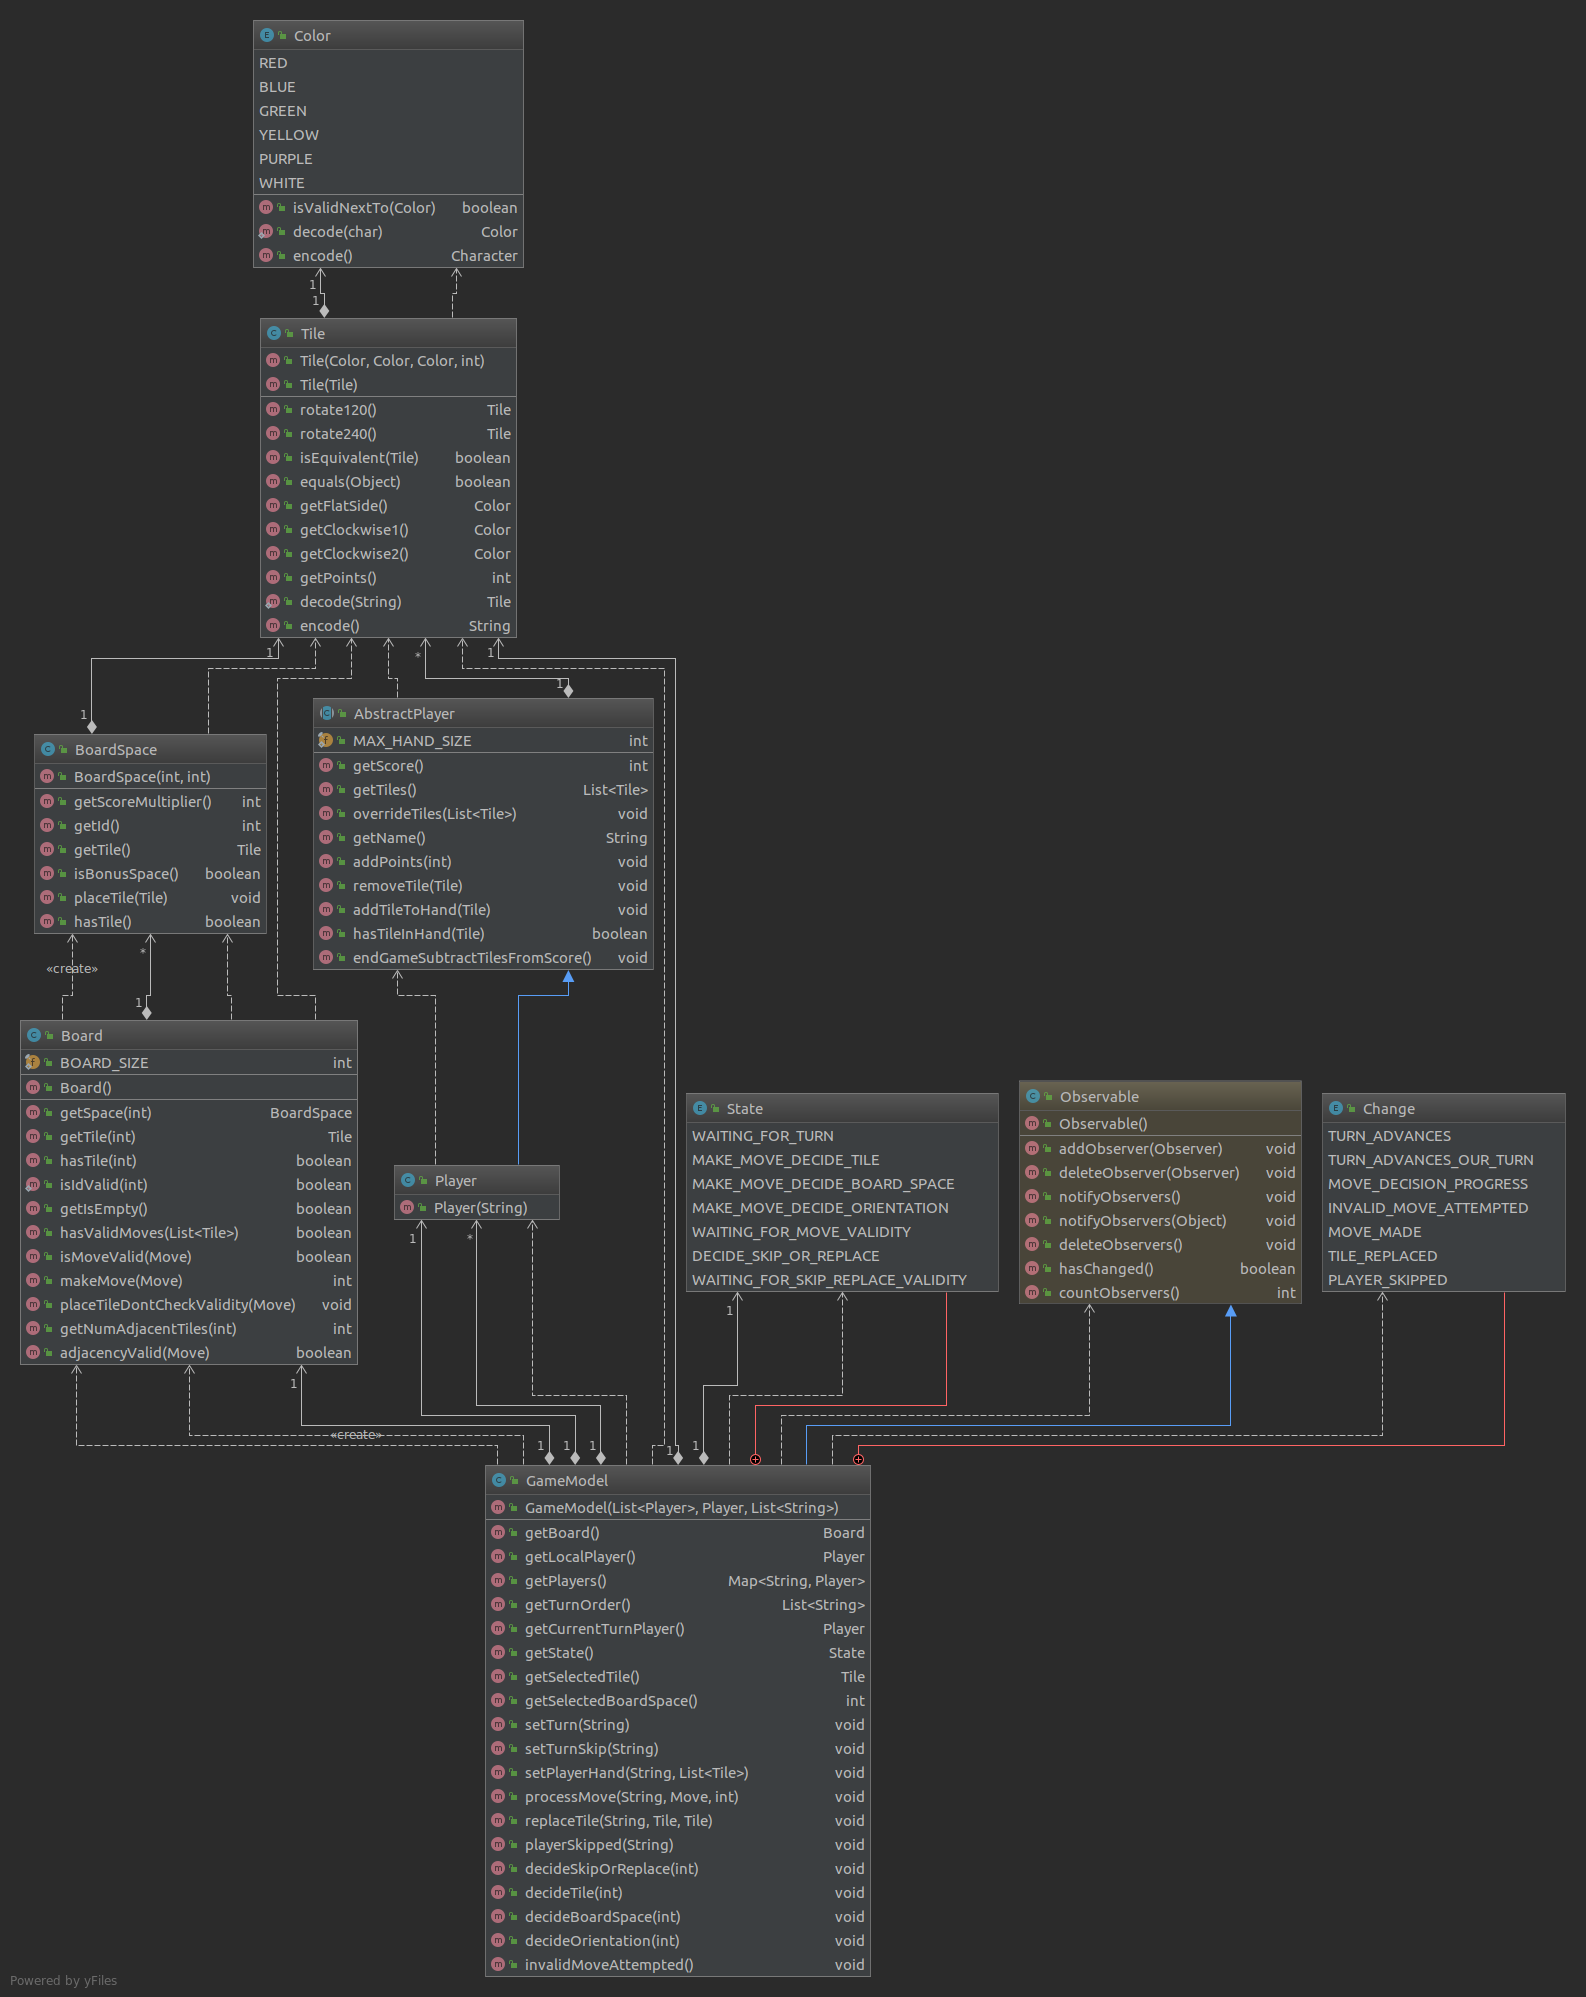
\includegraphics[width=\textwidth]{GameModel.png}
            \caption{Class diagram of the GameModel and the other self-defined classes it contains.}
            \label{fig:modelDiagram}
        \end{center}
    \end{figure}


\end{document}
